\documentclass[UTF8]{ctexart}   %指定文档的类型为 ctexart 使用 UTF-8 编码格式
\usepackage{ctex}               %调用ctex字库
\usepackage{graphicx}           %调用graphicx包库,用于插入图片
\usepackage{amsmath}            %调用amsmath包库,为基础数学包库,用在mathabx之前否则报错
\usepackage{mathabx}            %调用mathabx包库,用于 \bucause 、\therefore、的数学符号


\setCJKmainfont{SimSun}         %设置主要字体为宋体(SimSun)

\newcommand{\stxs}{\CJKfamily{SimSun}\fontsize{12pt}{18pt}\selectfont}
                                %定义命令 \newcommand{cmd}{def} 
                                %\stxs 设定为使用中文宋体12磅1.5倍行间距
\title{
    
\includegraphics[width=7.91cm,height=1.64cm]{logo.png}
                                %插入图片HBLGXY.png 设置图片宽7.91cm 高1.64cm
    \\
    \textbf{\CJKfamily{黑体}\fontsize{26pt}{39pt} 半导体物理与器件---问答题}
                                %使用加粗黑体26磅1.5倍行距
}

\author{                        %作者信息
    背包客/落云\\                %这东西不重要之前用过的一用户名而已
    Apy6631@outlook.com         %显然是一份邮箱
}

\date{\today}                   %文本创作时间 \today 为机器当前时间

\begin{document}                %正文开启的类似头文件的东西

\maketitle                      %生成标题/封面 在此之前的至 \title{title} 之后的均为设计不会生成

\thispagestyle{empty}           %设置此页不显示页码


\clearpage                      %可以理解为分页符

\thispagestyle{empty}

\tableofcontents                %自动生成目录

\clearpage

\section{前言}                  %设置标题
                                %标题等级:由高到低(由大到小排序)
                                %\section{title}
                                %\subsection{title}
                                %\subsubsection{title}

\begin{center}
    同上一个文本,写这个是为了练习一下LaTeX的使用,文本来自互联网及AI。
\end{center}
                                %\begin{center}
                                    %text
                                %\end{center}
                                %使文档text居中对齐

\setcounter{page}{1}            % 将页码计数器重置为 1

\clearpage                      %同上分页符

\section{正文}

\subsection{什么叫本征激发?温度越高,本征激发的载流子越多,为什么?试定性说明之。}

\stxs{解:在一定温度下,价带电子获得足够的能量($ \geq Eg $)被激发到导带成为导电电子的过程就是本征激发。其结果是在半导体中出现成对的电子-空穴对。
如果温度升高,则禁带宽度变窄,跃迁所需的能量变小,将会有更多的电子被激发到导带中。}

\subsection{试定性说明 $ Ge $ 、 $ Si $ 的禁带宽度具有负温度系数的原因。}

解:电子的共有化运动导致孤立原子的能级形成能带,即允带和禁带。温度升高,则电子的共有化运动加剧,导致允带进一步分裂、变宽;允带变宽,则导致允带与允带之间的禁带相对变窄。反之,温度降低,将导致禁带变宽。

因此, $ Ge $ 、 $ Si $ 的禁带宽度具有负温度系数。

\subsection{试指出空穴的主要特征。}

解:  空穴是未被电子占据的空量子态,被用来描述半满带中的大量电子的集体运动状态,是准粒子。主要特征如下:

\begin{table}[h]

    \begin{tabular}{ c l }

        A & 荷正电:$ +q $\\
        B & 空穴浓度表示为$ p $ (电子浓度表示为$ n $)\\
        C & $ E_{P} = - E_{n} $\\
        D & $ m_{P}^{*} = - m_{n}^{*} $\\

    \end{tabular}

\end{table}

                                %\begin{table}[h]
                                    %
                                %\end{table}
                                %{table}类似于提前占个座,[h]是定位
                                %\begin{tabular}{l s c}
                                    %
                                %\end{tabular}
                                %{tabular}是建立表格,{l c s}则指明了表格为三列,每列对应的对齐方式

\clearpage                      %同上分页符

\subsection{简述 $ Ge $ 、 $ Si $ 和 $ GaAS $ 的能带结构的主要特征。}

\begin{table}[h]
    \caption{ $Ge$、$Si$:}     
    \begin{tabular}{ c l }
    
        (a) & $E_{g} (Si:0K) = 1.21 eV ; E_{g} (Ge:0K) = 1.170 eV $\\
        (b) & 间接能隙结构 \\
        (c) & 禁带宽度 $ E_{g} $ 随温度增加而减小   
 
    \end{tabular}

\end{table}

\begin{table}[h]
    \caption{ $ GaAs $ }        %给表格命名
    \begin{tabular}{ c l }
        (a) & $E_{g}( 300 K)= 1.428 eV ;    E_{g} ( 0 K ) = 1.522 eV $ \\
        (b) & 直接能隙结构;\\
        (c) & Eg负温度系数特性: $ \frac{ \mathrm{d} E_{g} }{ \mathrm{d} T }  = -3.95 \times 10 ^{-4}eV/K$

    \end{tabular}
\end{table}

\clearpage                      %同上分页符

\subsection{
    某一维晶体的电子能带为
\begin{equation*}
    E(k) = E_{0}[ 1 - 0.1 \cos( k \alpha ) - 0.3 \sin( k \alpha )]
\end{equation*} 
其中$E_{0} = 3 eV $,晶格常数$ a = 5 \times 10^{-11} m $。\\
求:}

                                %\begin{equation}
                                    %
                                %\end{equation}
                                %做公式,默认自动编号,若想取消编号则在equation后加*

\subsubsection{能带宽度;}

由题意得:
\begin{equation}
    \frac{\mathrm{d}E}{\mathrm{d}k} = 0.1 \alpha E_{0}[ \sin( k \alpha ) -3 \cos( k \alpha ) ]
\end{equation}

\begin{equation}
    \frac{\mathrm{d}E^{2}}{\mathrm{d^{2}}k} = 0.1 \alpha ^{2} E_{0} [ \cos( k \alpha ) + 3 \sin( k \alpha ) ]
\end{equation}
令$ \frac{\mathrm{d} E }{\mathrm{d} k } = 0 $,得 $ tg (k\alpha)= \frac{1}{3} $

$ \therefore k_{1} \alpha = 18.4349 ^{\circ} ; k_{2} \alpha = 198.4349 ^{\circ} $

当$ \therefore k_{1} \alpha = 18.4349 ^{\circ} $ , $ \frac{\mathrm{d} E ^{2} }{\mathrm{d ^{2} k}} = 0.1 \alpha ^{2} E_{0} ( \cos18.4349 + 3 \sin18.4349 ) =2.88 \times 10^{-40} > 0 $ , 对应能带极小值;

当$ \therefore k_{2} \alpha = 198.4349 ^{\circ} $ , $ \frac{\mathrm{d} E ^{2} }{\mathrm{d ^{2} k}} = 0.1 \alpha ^{2} E_{0} ( \cos198.4349 + 3 \sin198.4349 ) =2.88 \times 10^{-40} < 0 $ , 对应能带极大值.

则能带宽度 $ \Delta E = E_{max} - E_{min} = 1.1384 eV $

                                %\because \therefore 是数学中的 因为、所以 就是那三个点
                                %这两者的使用要依赖于两个包库{amsmatha}、{mathabx}
                                %{mathabx}的调用需在{amsmatha}之后

\subsubsection{能带底和能带顶的有效质量。}

则  
$
    \left\lbrace 
        \begin{aligned}
            & {( m_{n} ^{*})_{\text{带底}} = [ \frac{1}{h^{2}} ( \frac{\mathrm{d} E^{2}}{ \mathrm{d^{2}} k})]^{-1} = [\frac{2.28 \times 10 ^{-40}}{(6.625 \times 10^{-34})^{2}}]^{-1} =1.925 \times 10^{-27} (kg) }  \\
            & {( m_{n} ^{*})_{\text{带顶}} = [ \frac{1}{h^{2}} ( \frac{\mathrm{d} E^{2}}{ \mathrm{d^{2}} k})]^{-1} = [\frac{2.28 \times 10 ^{-40}}{(6.625 \times 10^{-34})^{2}}]^{-1} =1.925 \times 10^{-27} (kg) }
        \end{aligned}
    \right .
$
答:能带宽度约为 $ 1.1384 Ev $,能带顶部电子的有效质量约为$ 1.925 \times 10 - 27 kg $,能带底部电子的有效质量约为 $ - 1.925 \times 10 - 27 kg $。

                                %\left\lbrace-\左\左花括号 \right.-\右\括号结束
                                %\left\lbrace-\左\左花括号 \right\rbrace-\右\右括号结束
                                %aligned 环境的基本语法如下:
                                %\begin{aligned}
                                %    <公式1> \\
                                %    <公式2> \\
                                %    ...
                                %\end{aligned}
                                %表示两个公式,第一个公式和第二个公式的等号对齐
                                %以经典的 \\  换行

\clearpage                      %同上分页符

\subsection{空间电荷区是怎样形成的。画出零偏与反偏状态下pn结的能带图。}

\begin{figure}[ht]
    \centering
    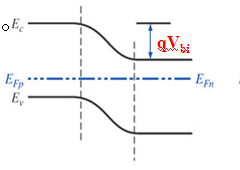
\includegraphics{PN0.png}
    \caption{PN节零偏时的结构图}
    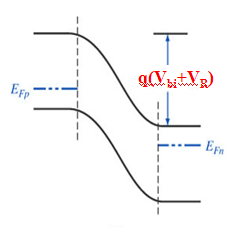
\includegraphics{PN1.png}
    \caption{PN节反偏时的结构图}
\end{figure}

                                %\begin{figure}[ht]                 -经典占位
                                %    \centering                     -指明居中
                                %    \includegraphics{name.jpg}     -图片存储路径图片名(最好和tex文件处于同一路径下)
                                %    \caption{text}                 -将图片命名为text
                                %    ...                            -显然可以重复插入多张图片
                                %\end{figure}

\clearpage                      %同上分页符

\section{结语}

\stxs{
     \hspace{2em}{此处首行缩进2字符}
     \hspace{2em}{连续使用是这种效果,然而}

     \hspace{2em}{空一空行继续使用会是这种效果。}

     此处首行缩进2字符连续使用是这种效果,然而空一空行继续使用会是这种效果。
                                %\stxs 为本文自定义的命令,详情请看上文|7行
                                %\hspace{size}{text}
                                %text文本首行缩进size个字符
                                %LaTeX中以换行判定分段 所以若连续使用时需要使用空行分段
}
\end{document}                  %结束document(正文)
